\documentclass[12pt]{article}
\usepackage[utf8]{inputenc}
\usepackage{amsmath}
\usepackage{listings}
\usepackage{graphicx}
\title{CS 472 Fall 2011 \\
     Project 1A}
\author{Colby Blair}
\date{Due September 14th, 2011}

\begin{document}
\maketitle

\begin{abstract}
Evolutionary Computation is the study of combonational logic, that can often provide reasonable solutions to
intractably complex problems. In Evolutionary Computation, there are many different approaches to optimizing a solution for a problem. Different approaches often result in better result, depending on the problem to be solved. This project considers the Spherical / Schwefel function, and tries to solve it using a Genetic Algorithm (GA).

In this report, it will be found that some solutions work badly, some work much better, and some are clear winners over the rest. Specifically, this report will find that a Generational Rank Selection with Elitism was better than the other tested solutions. In testing methods, the changes can be subtle, but can make all the difference. This report will talk about when and why these solution would fail. It will also discuss other possible solution methods, and why they were not used here. Finally, this report will identify what 
improvements could be made, and where parallelism can be achieved in harder problems.
\end{abstract}
\pagebreak

\part{Algorithm Descriptions}
\label{part:alg_desc}

A Genetic Algorithm (GA) create a \textbf{population} of individuals, each of which have attributes to try to solve a problem. Their correctness will be measure with a \textbf{fitness function}. The best of these individuals are found with \textbf{selection}, their attributes are combined using \textbf{crossover}, and a child is produced from this. Each child is then slightly \textbf{mutated}, or its attributes changed. This results in new individuals in the population, and the whole process is started again.

The \textbf{population} for all the GA methods in this report is represented as a list of vectors. The \textbf{initial population} has random values set in the attributes vector (x) for every individual (see Figure \ref{uniform_mutation}):
\begin{figure}[!h]
        \begin{center}
		\begin{tabular}{r l}
	                $ P = i_1, i_2, ... i_j $	& \\
								& where \\
								& $ i_n $ is a vector of floats ( $ = x_1, x_2, ... x_y $ ) \\
								& $ j = 500 $ \\
								& $ y = 30 $ \\
								& $ x_n = [-5.12, 5.12] $
		\end{tabular} 
               \caption{The representation of the population}
                \label{population}
        \end{center}
\end{figure}

All of the GA methods here will use the Spherical / Schfewel function to calculate their \textbf{fitness}. The GA's will then try to find the minimum fitnesses, or the individual(s) that attributes add up to 0:
\begin{figure}[!h]
        \begin{center}
		\begin{tabular}{r l}
			$ f(i_j) = $			&	$ \sum_{y=1}^{1}x_y^2	$ for $ i_j $ \\
								& \\
								&	where \\
								&	$ x_y = [-5.12, 5.12 ] $ \\
		\end{tabular} 
               \caption{The fitness function}
                \label{fitness}
        \end{center}
\end{figure}

For \textbf{selection}, the two individuals with the smallest fitnesses will be selected. For computational reasons, this report was able to survey the entire population instead of selecting small random subsets. No performance gain was needed yet.

The \textbf{crossover} function will take two individuals $ i_a, i_b $, and return a child individual, which has a mix of attributes ( $x_n $ values) from each parent. Specifically, \textbf{one point crossover} is used:
\begin{figure}[!h]
        \begin{center}
		\begin{tabular}{r l}
	                $ crossover(i_a, i_b) = $ & \\
			& $ x_{i_a}[1:n], x_{i_b}[n:length(i_b) $ x values for the new child individual \\
								& where \\
								& $ n = $ a random integer from $ 1 ... $ the length of $i_b$
		\end{tabular} 
               	\caption{One point crossover}
                \label{one_crossover}
        \end{center}
\end{figure}

Finally, a simple \textbf{uniform mutation} function was used. For any new child created from crossover, it would then be mutated before insertion into a new population:
\begin{figure}[!h]
        \begin{center}
		\begin{tabular}{r l}
	                $ mutate(x_i[n]) $ 		& $ = $ random value in the domain $ [-5.12, 5.12] $\\
								& where \\
								& $ n = $ a random integer from $ 1 ... $ the length of $x_i$
		\end{tabular} 
               	\caption{Uniform mutation}
                \label{uniform_mutation}
        \end{center}
\end{figure}

\section{Steady State}
The \textbf{steady state} algorithm used the \textbf{population} described in Figure \ref{population}, the \textbf{fitness} function described in Figure \ref{fitness}, the \textbf{selection} described in Part \ref{part:alg_desc}, the \textbf{crossover} described in Figure \ref{one_crossover}, and the \textbf{mutation} described in Figure \ref{uniform_mutation}.

The flow of converging on a solution is as follows:
\begin{itemize}
	\item while min fitness of population is greater than 0.00
	\begin{itemize}
		\item calculate current fitnesses
		\item select 2 individuals (parents) with minimum fitnesses
		\item create new child from the 2 parents using one point crossover
		\item mutate the new child using uniform mutation
		\item replace the individual in the population with the max fitness, with the new child
	\end{itemize}
\end{itemize}


\section{Generational}
\label{sec:gen}
The \textbf{generational} algorithm used the \textbf{population} described in Figure \ref{population}, the \textbf{fitness} function described in Figure \ref{fitness}, the \textbf{selection} described in Part \ref{part:alg_desc}, the \textbf{crossover} described in Figure \ref{one_crossover}, and the \textbf{mutation} described in Figure \ref{uniform_mutation}.

The flow of converging on a solution is as follows:
\begin{itemize}
	\item while min fitness of population is greater than 0.00
	\begin{itemize}
		\item calculate current fitnesses
		\item select 2 individuals (parents) with minimum fitnesses
		\item create new child from the 2 parents using one point crossover
		\item for every individual in the population
			\begin{itemize}
				\item mutate a copy of the new child using uniform mutation, making a new mutant child
				\item replace the individual with the new mutant child
			\end{itemize}
	\end{itemize}
\end{itemize}


\section{Generational with Elitism}
The \textbf{generational with elitism} algorithm used the \textbf{population} described in Figure \ref{population}, the \textbf{fitness} function described in Figure \ref{fitness}, the \textbf{selection} described in Part \ref{part:alg_desc}, the \textbf{crossover} described in Figure \ref{one_crossover}, and the \textbf{mutation} described in Figure \ref{uniform_mutation}. This GA used \textbf{elitism}; it kept the 2 best individuals in the population by copying them into every new genertion.

The flow of converging on a solution is very similar to Section \ref{sec:gen}, as follows:
\begin{itemize}
	\item while min fitness of population is greater than 0.00
	\begin{itemize}
		\item calculate current fitnesses
		\item select 2 individuals (parents) with minimum fitnesses
		\item create new child from the 2 parents using one point crossover
		\item for every individual in the population
			\begin{itemize}
				\item mutate a copy of the new child using uniform mutation, making a new mutant child
				\item replace the individual with the new mutant child
			\end{itemize}
		\item replace the 2 max fitnesses in the population with the 2 parents
	\end{itemize}
\end{itemize}


\part*{Results}

\section{Steady State}
\begin{figure}[!h]
        \begin{center}
		\includegraphics[width=30mm]{images/ss/ind_101.pdf}
		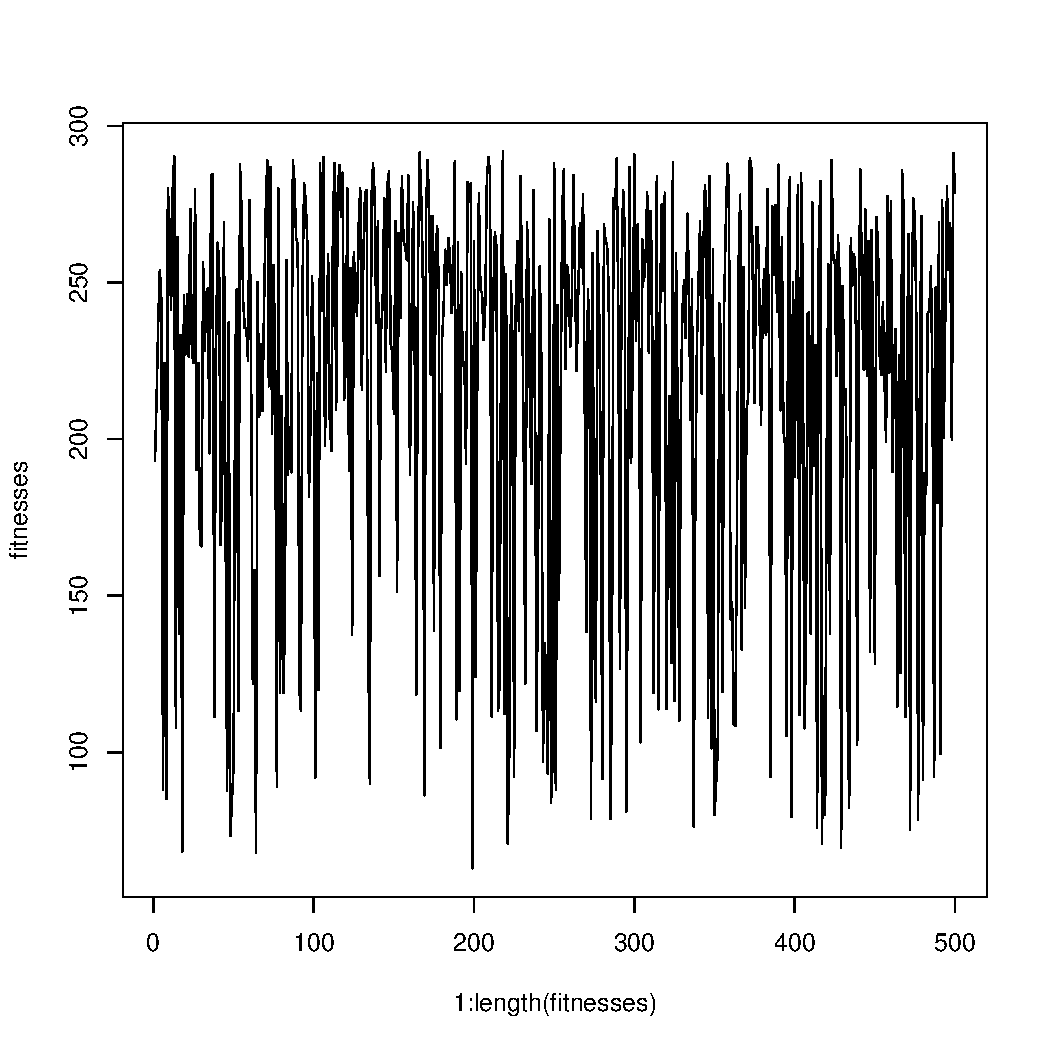
\includegraphics[width=30mm]{images/ss/ind_110.pdf}
		\includegraphics[width=30mm]{images/ss/ind_404.pdf}
		\includegraphics[width=30mm]{images/ss/ind_505.pdf}
               	\caption{Population fitnesses at 100, 110, 400, and 500 iterations, respectively}
                \label{ss_pop_fit}
        \end{center}
\end{figure}

\begin{figure}[!h]
        \begin{center}
		\includegraphics[width=30mm]{images/ss/avg_101.pdf}
		\includegraphics[width=30mm]{images/ss/avg_1717.pdf}
		\includegraphics[width=30mm]{images/ss/avg_2222.pdf}
		\includegraphics[width=30mm]{images/ss/avg_2525.pdf}
               	\caption{Average population fitnesses at 100, 1717, 2222, and 2525 iterations, respectively, at 100 iteration wide snapshots}
                \label{ss_avg_pop_fit}
        \end{center}
\end{figure}

The steady state GA never converged to 0.00, and at 2582 iterations (2 minutes 54 seconds), here was the lowest individual:
\scriptsize
\begin{lstlisting}
[1] "2582  - Avg fitness: 1.8227024 min: 0.4418"
[1]  0.04  0.00  0.00 -0.09  0.02  0.01  0.02 -0.26 -0.13  0.25  0.02  0.00
[13]  0.01  0.02  0.20  0.22 -0.24  0.13 -0.04 -0.01  0.12  0.08 -0.13 -0.13
[25]  0.06 -0.19 -0.07  0.05 -0.11 -0.07
\end{lstlisting}
\normalsize

\section{Generational}
\begin{figure}[!h]
        \begin{center}
		\includegraphics[width=30mm]{images/gen/ind_101.pdf}
		\includegraphics[width=30mm]{images/gen/ind_120.pdf}
		\includegraphics[width=30mm]{images/gen/ind_130.pdf}
		\includegraphics[width=30mm]{images/gen/ind_505.pdf}
               	\caption{Population fitnesses at 100, 120, 130, and 505 iterations, respectively}
                \label{ss_pop_fit}
        \end{center}
\end{figure}

\begin{figure}[!h]
        \begin{center}
		\includegraphics[width=30mm]{images/gen/avg_101.pdf}
		\includegraphics[width=30mm]{images/gen/avg_120.pdf}
		\includegraphics[width=30mm]{images/gen/avg_130.pdf}
		\includegraphics[width=30mm]{images/gen/avg_505.pdf}
               	\caption{Average population fitnesses at 100, 120, 130, and 505 iterations, respectively, at 100 iteration wide snapshots}
                \label{ss_avg_pop_fit}
        \end{center}
\end{figure}

The generation GA never converged to 0.00, and at 2582 iteration (3 minutes 54 seconds), here was the lowest individual:
\scriptsize
\begin{lstlisting}
[1] "2582  - Avg fitness: 8.3794016 min: 0.0122" 
[1] -0.02  0.01  0.00 -0.04  0.00  0.01  0.00 -0.01 -0.01  0.00  0.00 -0.01
[13] -0.01 -0.01  0.00 -0.01 -0.02  0.02  0.01 -0.02 -0.02 -0.01  0.01  0.01
[25]  0.02 -0.01 -0.02  0.00  0.07  0.04
\end{lstlisting}
\normalsize


\pagebreak


\section{Generational with Elitism}
\begin{figure}[!h]
        \begin{center}
		\includegraphics[width=30mm]{images/gen_elite/ind_101.pdf}
		\includegraphics[width=30mm]{images/gen_elite/ind_120.pdf}
		\includegraphics[width=30mm]{images/gen_elite/ind_130.pdf}
		\includegraphics[width=30mm]{images/gen_elite/ind_404.pdf}
               	\caption{Population fitnesses at 100, 120, 130, and 404 iterations, respectively}
                \label{ss_pop_fit}
        \end{center}
\end{figure}

\begin{figure}[!h]
        \begin{center}
		\includegraphics[width=30mm]{images/gen_elite/avg_101.pdf}
		\includegraphics[width=30mm]{images/gen_elite/avg_120.pdf}
		\includegraphics[width=30mm]{images/gen_elite/avg_130.pdf}
		\includegraphics[width=30mm]{images/gen_elite/avg_140.pdf}
               	\caption{Average population fitnesses at 100, 120, 130, and 140 iterations, respectively, at 100 iteration wide snapshots}
                \label{ss_avg_pop_fit}
        \end{center}
\end{figure}

The generational with elitism GA converged at 0.00 around 462 iterations (50 seconds), here was the lowest individual right before converging:
\scriptsize
\begin{lstlisting}
[1] "461  - Avg fitness: 8.479347 min: 1e-04"
 [1]  0.00  0.00  0.00  0.00  0.00  0.00  0.00  0.00  0.00  0.00  0.00  0.00
[13]  0.00  0.00  0.00  0.00  0.00  0.00  0.00  0.00  0.00  0.00  0.00 -0.01
[25]  0.00  0.00  0.00  0.00  0.00  0.00
\end{lstlisting}
\normalsize


\part{Conclusion}
\section{Algorithms}
\textbf{Steady state} preserves existing populations, which could do well when many local minimums could surround a global minimum. However, it takes longer to converge on a single minimum, and in the case of the Spherical / Schwefel function, there is only one minimum. This makes this steady state a bad choice.

\textbf{Generational} is completely disruptive of existing populations, because it regenerates a new population every generation. This leads to a much faster convergence towards 0.00, but the uniform mutation delays this convergence, because it doesn't scale down its rate. This leads to wildly worse mutated childs when the overall population has good fitnesses, and therefore most mutated childs are bad and a waste of time. 

This also lead to the incorrect mutation of the best individual's DNA, which was unfavorable. One solution that my classmates tries was scaling down mutations closer to convergence, but I tried a different approach with the next GA.

The clear winner here was the \textbf{generational with elitism} GA, because it actually converged to 0.00, and because it did so in under a minute. It didn't hang on to bad individuals like steady state did, but it kept the best ones around through elitism, unlike the simple generational GA. It also did not mutate the best individual unfavorably, because of elitism. It probably won't be a winner, however, with more variatable algorithms; in which case, steady state may be a good choice.

\section{Performance}
The algorithms here were left to a lot of brute force, because the environment made it practical. Sampling the population would be a better choice if the process time of the fitness algorithm increase. Also, sometimes the fitness algorithm was needlessly recalculated. 

Another topic is \textbf{parallelism}. Data dependency prevents \textbf{task parallelism} on the optimization (although it could perhaps be pipeline parallelized), the way the above GA's seperate the fitness calculation could lead to true task parallelization on the fitness calculation. This wouldn't be as adventagious in the generational GA (every generation only needs 2 new fitness calculations), but would be much more adventagious in the simple state GA (where every new generation needs all fitnesses recalculated). 

The Spherical / Schwefel function does not justify the communication overhead for parallelization, but if we write GAs in the future that need a lot of fitness recalcuation, like steady state, then future reports will implement parallelization. 

\end{document}
